%!TEX root = master.tex

\section{Language features}


\begin{frame}
  \frametitle{java.lang.Object}

  \begin{itemize}
    \item Java is object-oriented, so everything is/should be an object!
  \end{itemize}
  \vspace{1cm}
  \begin{center}
    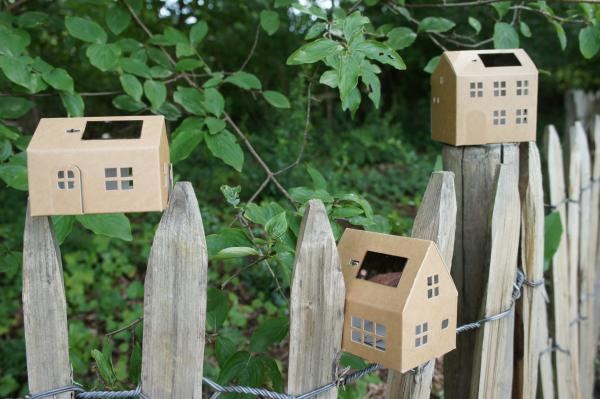
\includegraphics[width=0.4\textwidth]{fig/objects}
  \end{center}
\end{frame}


\begin{frame}
  \frametitle{java.lang.Object}

  \begin{itemize}
    \item Except byte, boolean, short, char, int, long, float, double
    \vspace{1cm}
    \item They are primitive (of course...)
  \end{itemize}
\end{frame}


\begin{frame}
  \frametitle{java.lang.generics.*}
  Java has generics:
  \vspace{0.25cm}
  \begin{itemize}
    \item Useful to write generic algorithms
    \vspace{0.4cm}
    \item Implement container classes (lists, maps, etc.)   
    \vspace{0.4cm}
    \item Generic compile errors can be hard to solve, but not as bad as C++
  \end{itemize}
\end{frame}


\begin{frame}
  \frametitle{java.lang.generics.*}
  Drawback: Only works with reference types =(
\end{frame}


\begin{frame}
  \frametitle{java.lang.generics.*}
	\begin{center}
	    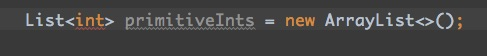
\includegraphics[width=0.8\textwidth]{fig/primarray}    
	\end{center}

	\begin{center}
	    
\includegraphics[width=0.5\textwidth]{fig/primitives}    
	\end{center}
\end{frame}


\begin{frame}
  \frametitle{java.lang.generics.*}
 \begin{itemize}
    \item Might change with Java 9 (2016) or Java 10 (2018)
    \vspace{0.4cm}
    \item HotSpot JEPs \& JSRs: Project Valhalla, Project Panama
  \end{itemize}  
\end{frame}


\begin{frame}
  \frametitle{java.lang.*}

 \begin{itemize}
    \item Code can only live in Classes
    \vspace{0.3cm}
    \item Syntactically close to C/C++ (Braces, etc.)
    \vspace{0.3cm}
    \item Reflective
    \vspace{0.3cm}
    \item Built-in support for multithreading (synchronized keyword, etc.)
    \vspace{0.3cm}
    \item Built-in support for serialization (transient keyword, etc.)
    \vspace{0.3cm}
    \item No multiple inheritance, all methods are virtual and overloadable
    \vspace{0.3cm}
    \item Since JDK8: Native support for lambda's and functional programming =)
  \end{itemize}  
  
\end{frame}


\begin{frame}
  \frametitle{java.util.*}

 \begin{itemize}
    \item Well defined concurrency libraries, arguably the best ones out there
    \vspace{0.3cm}
    \item Very performant network library implementation
    \vspace{0.3cm}  
    \item Therefore heavily used in backend systems (financial, social media, etc.)
    \vspace{0.3cm}
    \item Large number of open-source libraries
    \vspace{0.3cm}
    \item Gigantic community
  \end{itemize}  
  
\end{frame}


\begin{frame}
  \frametitle{java.lang.impl.HotSpot}
  \begin{itemize}
    \item Oracle's reference implementation is the HotSpot JVM
    \vspace{0.3cm}
    \item ByteCode interpreter
    \vspace{0.3cm}    
    \item JIT	(state-of-the-art, gets much better in Java 9)
    \vspace{0.3cm}    
    \item GC 	(state-of-the-art, even concurrent)    
  \end{itemize}
\end{frame}

\begin{frame}
  \frametitle{java.lang.impl.HotSpot}

  Runtime characteristics:
  \vspace{0.25cm}    
  \begin{itemize}
    \item It takes a while to warm up the JIT
    \vspace{0.3cm}    
    \item Learns about code-flow, dead-code elimination
    \vspace{0.3cm}    
    \item Dynamic stack allocation (through escape-analysis)
    \vspace{0.3cm}    
    \item Dynamic code optimizations
    \vspace{0.3cm}
    \item At some point very, very fast
    \vspace{0.3cm}
    \item Relatively high memory usage
    \vspace{0.3cm}
    \item In some situations on-par with C/C++ (no flame-war intended)
    \vspace{0.3cm}
    \item Conclusion: Perfect for long running, backend server applications
  \end{itemize}
\end{frame}